\documentclass[11pt,aspectratio=169]{beamer}

% --- Tema og fonte ---
\usetheme{Madrid}
\usefonttheme{serif}
% --- Farver ---
\definecolor{myteal}{RGB}{14,71,57}
\setbeamercolor{title}{fg=white}
\setbeamercolor{frametitle}{fg=white,bg=myteal}
\setbeamercolor{block title}{fg=white,bg=myteal}
\setbeamercolor{block body}{bg=myteal!10}
\setbeamercolor{normal text}{fg=myteal}
\setbeamercolor{background canvas}{bg=white}
\setbeamercolor{structure}{fg=myteal}
\setbeamercolor{palette primary}{fg=white,bg=myteal}
\setbeamercolor{palette secondary}{fg=white,bg=myteal!80}
\setbeamercolor{palette tertiary}{fg=white,bg=myteal!60}
\setbeamercolor{author in head/foot}{fg=white,bg=myteal}
\setbeamercolor{title in head/foot}{fg=white,bg=myteal!80}
\setbeamercolor{date in head/foot}{fg=white,bg=myteal!60}
\setbeamercolor{titlelike}{fg=myteal}
\setbeamercolor{section in toc}{fg=myteal}
\setbeamercolor{item}{fg=myteal}
% --- Sprog og encoding ---
\usepackage[utf8]{inputenc}
\usepackage[danish]{babel}
\usepackage[T1]{fontenc}
\usepackage{lmodern}
% --- Matematik ---
\usepackage{amsmath,amsfonts,amssymb}
% --- Grafik og layout ---
\usepackage{graphicx}
\usepackage{ragged2e}
\usepackage{booktabs}
\usepackage{arydshln}
\usepackage[most]{tcolorbox}
% --- Ikoner og figurer ---
\usepackage{fontawesome5}
\usepackage{tikz}
\usetikzlibrary{positioning,arrows.meta,shapes.geometric,calc}
\usepackage{circuitikz}
% --- Positionering ---
\usepackage[absolute,overlay]{textpos}
% --- CSV ---
\usepackage{csvsimple}
% --- Kildehenvisning nederst på slides ---
\setbeamercolor{framesource}{fg=gray,bg=white}
\setbeamerfont{framesource}{size=\scriptsize}
\newcommand{\framesource}[1]{%
  \begin{textblock*}{12cm}(0.5cm,8.6cm)
    \raggedleft
    \beamercolorbox[wd=\textwidth,rightskip=0.5cm]{framesource}{#1}
  \end{textblock*}
}
% --- Automatisk billedattribution ---
\csvreader[
  head to column names,
  no head
]{Billeder/billedkilder.csv}{}{}
\newcommand{\billedkilde}[1]{%
  \csvreader[
    head to column names,
    full filter=\ifcsvstrcmp{\filnavn}{#1}{\csvfilteraccept}{\csvfilterreject},
    no head
  ]{Billeder/billedkilder.csv}{}%
  {%
    \tiny\forfatter\ / Wikimedia Commons (\licens)%
  }%
}
% --- Boksstile til jagttid-sliden ---
\tcbset{
  gruppe/.style={
    enhanced,
    colback=white,
    colframe=myteal,
    coltitle=myteal,
    boxrule=0.8pt,
    dashed,
    sharp corners,
    fonttitle=\bfseries\large,
    attach boxed title to top left={yshift=-2mm,xshift=3mm},
    boxed title style={colback=white,colframe=white,boxrule=0pt,sharp corners},
    top=1mm,left=1mm,right=1mm,bottom=1mm
  },
  felt/.style={
    enhanced,
    colback=white,
    colframe=myteal,
    boxrule=0.6pt,
    sharp corners,
    halign=center,
    valign=center,
    width=\linewidth,
    height=1.55cm,
    fit,
    fit algorithm=fontsize,
    fit basedim=7pt,
    boxsep=0.3mm,
    left=0.5mm, right=0.5mm, top=0.3mm, bottom=0.3mm
  },
  feltfri/.style={
    enhanced,
    colback=white,
    colframe=myteal,
    boxrule=0.6pt,
    sharp corners,
    halign=center,
    valign=center,
    width=\linewidth,
    boxsep=0.3mm,
    left=0.5mm, right=0.5mm, top=0.3mm, bottom=0.3mm,
    fontupper=\scriptsize
  }
}
% --- Matematiske operatorer ---
\DeclareMathOperator{\sen}{sen}
\DeclareMathOperator{\tg}{tg}
% --- Beamer-indstillinger ---
\setbeamertemplate{caption}[numbered]
\setbeamertemplate{navigation symbols}{}
% --- Forfatter ---
\author[Østerbro Jagttegn]{Østerbro Jagttegn \\ \textbf{Aleksander Sønder}}
% --- Hyperref (altid sidst) ---
\usepackage{hyperref}
\hypersetup{
  colorlinks=true,
  linkcolor=myteal,
  urlcolor=myteal,
  citecolor=myteal
}

\title{Modul 4 \\
Obligatorisk Jagttegnskursus \\ @ Microsoft 18:00-21:00}
\date{\today}

\begin{document}

% Titelside
\begin{frame}
  \titlepage
\end{frame}

% Indholdsfortegnelse (valgfri)
\begin{frame}{Program}
  \tableofcontents
\end{frame}

\section{Jagtudøvelse}

\begin{frame}
  \vspace{3em}
  \begin{center}
    {\LARGE \textbf{Bekendtgørelse af lov om jagt og vildtforvaltning}} \\
    \vspace{1em}
    LBK nr 639 af 26/05/2023, §§ 13-32
  \end{center}
\end{frame}

\begin{frame}{Jagtretten – grundregler (§13–§15)}
    \begin{itemize}
        \item \textbf{§13}: Ingen må jage uden jagtret – medmindre samtykke fra jagtberettiget
        \item \textbf{§14}: Jagtretten tilkommer ejendommens ejer
          \begin{itemize}
            \item På ferske vande (uden særlig ejendomsret): Ejerne af tilstødende ejendomme (nærmeste del)
            \item Gælder ikke hvis ældre rettigheder giver retten til andre
          \end{itemize}
        \item \textbf{§15}: Fast bopæl i DK → ret til ikke-erhvervsmæssig jagt på fiskeriterritoriet (fra højeste vandstandslinje)
          \begin{itemize}
            \item Gælder ikke hvis ældre ret til tilgrænsende landarealer
            \item Undtagelse: EU/EØS-borgere med tilknytning til DK
          \end{itemize}
    \end{itemize}
\end{frame}

\begin{frame}{Jagtretten – offentlig vej og tilegnelse (§16–§17)}
    \begin{itemize}
        \item \textbf{§16}: Forbud mod jagt på/fra offentlig vej eller sti
          \begin{itemize}
            \item Tilladt at tilegne sig beskudt vildt, der falder på vej/sti fra egen grund
          \end{itemize}
        \item \textbf{§17}: Beskudt vildt på egen grund → må ikke tilegnes hvis det falder på anden grund
          \begin{itemize}
            \item Underret snarest ejer/jagtberettiget
          \end{itemize}
    \end{itemize}
\end{frame}

\begin{frame}{Arealgrænser og minimumskrav (§18)}
    \begin{itemize}
        \item \textbf{§18}: Minimum 1 ha sammenhængende areal til jagt (vej/jernbane krydses OK)
          \begin{itemize}
            \item Fra 1 - 5 ha: Kun ejer + husstand (eller brugsret-indehaver + husstand)
            \item Aftale med tilgrænsende arealer → kan overstige grænser (naboaftale)
            \item Øer mindre end 1 ha: OK hvis jagt tilladt på omgivende fiskeriterritorium
            \item Fælleseje (flere end 4 ejere): Skriftlig aftale + 3/4 tilslutning
          \end{itemize}
    \end{itemize}
\end{frame}


\begin{frame}{Afstande, overdragelse og ældre rettigheder (§19–§21)}
    \begin{itemize}
        \item \textbf{§19}: Ingen skud inden for 50 m fra beboelsesbygninger (uden samtykke)
          \begin{itemize}
            \item På fiskeriterritoriet: 100 m fra sommerhusområde / 500 m fra byzone
          \end{itemize}
        \item \textbf{§20}: Jagtretten kan ikke afhændes særskilt/varigt fra ejendomsretten
          \begin{itemize}
            \item Overdragelse: Max 30 år ad gangen
            \item Ved brugsret-overdragelse: Jagtretten følger med (medmindre aftalt andet)
          \end{itemize}
        \item \textbf{§21}: Ældre rettigheder → ejer kan kræve afløsning (kapitaliseret jagtleje)
    \end{itemize}
\end{frame}



\begin{frame}{Jagtetik, sikkerhed og unge jægere (§22–§23)}
    \begin{itemize}
        \item \textbf{§22}: Ingen må jage på en måde, der
          \begin{itemize}
            \item udsætter vildtet for unødige lidelser
            \item skader personer, husdyr eller genstande eller udsætter personer for nærliggende fare
            \item medfører haglnedfald på anden persons bolig, have eller gårdsplads
          \end{itemize}
        \item \textbf{Stk. 2}: Personer under 18 år (med gyldigt jagttegn) må kun jage i følge med en person over 18 år (med gyldigt jagttegn)
        \item \textbf{§23}: Nedlæggelse/ombringelse af vildt må kun ske med skydevåben
          \begin{itemize}
            \item Rovfugle og ugler må ikke anvendes til jagt
            \item Jagt må ikke ske med levende lokkedyr
          \end{itemize}
    \end{itemize}
\end{frame}

\begin{frame}{Våbenkrav, hunde og jagt fra køretøj/fartøj (§24–§26)}
    \begin{itemize}
        \item \textbf{§24}: Ved jagt med glatløbet haglgevær på ikkeklovbærende vildt (på/fra landarealer, rør- og sivbevoksninger) skal egnet apporterende hund medbringes
        \item \textbf{§25}: Jagt må ikke finde sted fra motordrevet køretøj eller luftfartøj
        \item \textbf{§26}: Jagt fra motordrevet fartøj må ikke finde sted på søer og andre ferske vande
        \item \textbf{§23 stk. 4–6}: Ministeren fastsætter regler om
          \begin{itemize}
            \item tilladte våben/ammunition
            \item salg/medtagelse af visse ammunitionstyper
            \item brug af rovfugle, hjælpemidler, lokkemidler mv.
          \end{itemize}
    \end{itemize}
\end{frame}

\begin{frame}{Fodring, skjul, hegn og færdsel med våben (§28–§31)}
    \begin{itemize}
        \item \textbf{§28}: Udfodring af vildt med jagt for øje må ikke finde sted – vildt må ikke beskydes nær foderplads
          \begin{itemize}
            \item Ministeren kan fastsætte regler om fodring, foderpladser og placering
          \end{itemize}
        \item \textbf{§29}: Ministeren kan fastsætte regler om jagt fra platforme/kunstige skjul (inkl. forbud mod at medtage våben)
        \item \textbf{§30}: Hegn skal tillade ens passage af vildt fra begge sider (undtaget udsætningspladser, skovkulturer, veje/jernbaner)
        \item \textbf{§31}: Uvedkommende må ikke færdes med skydevåben/fangstredskaber på anden persons jagtgrund (undt. offentlige veje/stier)
          \begin{itemize}
            \item Gælder også i skove – kun på offentlige veje gennem skoven
            \item Naturbeskyttelseslovens adgangsregler giver ikke ret til at medbringe skydevåben/fangstredskaber
          \end{itemize}
    \end{itemize}
\end{frame}

\begin{frame}{Særlige jagtformer og anholdelsesbeføjelser (§27, §32)}
    \begin{itemize}
        \item \textbf{§27}: Ministeren kan fastsætte regler om jagtformer (herunder forbyde særlige former i bestemte områder)
        \item \textbf{§32}: Den jagtberettigede (eller dennes folk) må anholde enhver, der overtræder §13 (ulovlig jagt uden ret)
          \begin{itemize}
            \item Må føre den anholdte til politiet
            \item Samme beføjelse til arealet brugeren (selv uden jagtret) – skal underrette jagtberettiget
            \item Anholdte kan fratages skydevåben, redskaber og skudt/fanget vildt – afleveres straks til politiet (beslaglæggelse vurderes)
          \end{itemize}
    \end{itemize}
\end{frame}

\begin{frame}
  \vspace{3em}
  \begin{center}
    {\LARGE \textbf{Jagtudøvelse}
    }
    \\
    \vspace{1em}
    Bekendtgørelse om udsætning af vildt, jagtmåder og jagtredskaber
    \\
    \vspace{1em}
    BEK nr 1652 af 19/12/2017, Kapitel 2-5
  \end{center}
\end{frame}

\begin{frame}{Jagt i nærheden af indhegninger med hjorte (§4–§5)}
    \begin{itemize}
        \item \textbf{§4}: På ejendom med indhegnet hold af hjortedyr (jf. lov om hold af dyr)
          \begin{itemize}
            \item Vildtlevende individer af de opdrættede arter må \textbf{ikke} jages
            \item Gælder \textbf{i indhegningen} eller inden for \textbf{300 m} fra indhegningen
            \item Gælder også indhegninger, der er undtaget helt/delvist fra lov om hold af dyr (§19)
          \end{itemize}
        \item \textbf{§5}: På ejendom, hvor der \textbf{tidligere} har været holdt hjortedyr i indhegninger
          \begin{itemize}
            \item Hjortedyr må \textbf{ikke} jages \textbf{i indhegningen}
            \item Gælder hvis indhegningen (eller væsentlige dele) fortsat findes
          \end{itemize}
    \end{itemize}
\end{frame}



\begin{frame}{Jagt på fiskeriterritoriet – grundregler (§6)}
    \begin{itemize}
        \item \textbf{§6 stk. 1}: Den frie jagtret (jf. lovens §15) må kun udøves
          \begin{itemize}
            \item Fra flydende båd eller pram
            \item Fra areal, der grænser op til fiskeriterritoriet, hvor man har jagtret
          \end{itemize}
        \item \textbf{Stk. 2}: Færdsel med skydevåben under vadning på fiskeriterritoriet er \textbf{ikke tilladt}
        \item \textbf{Stk. 3} – Undtagelser (uanset stk. 1):
          \begin{itemize}
            \item Lovligt nedlagt vildt må indsamles ved vadning
            \item Rør- og sivbevoksninger må afdrives for vildt af den, der har jagtret på nærmeste tilgrænsende areal
          \end{itemize}
        \item \textbf{Stk. 4} – Vadning med skydevåben tilladt hvis:
          \begin{itemize}
            \item Skydevåbnet er \textbf{uladt}
            \item Vadning sker til/fra fartøj, ø eller holm med jagtret
            \item Ad korteste vej til sted, hvor våben lovligt kan medbringes (jf. §31)
          \end{itemize}
    \end{itemize}
\end{frame}

\begin{frame}{Fiskeriterritoriet}
    \begin{center}
        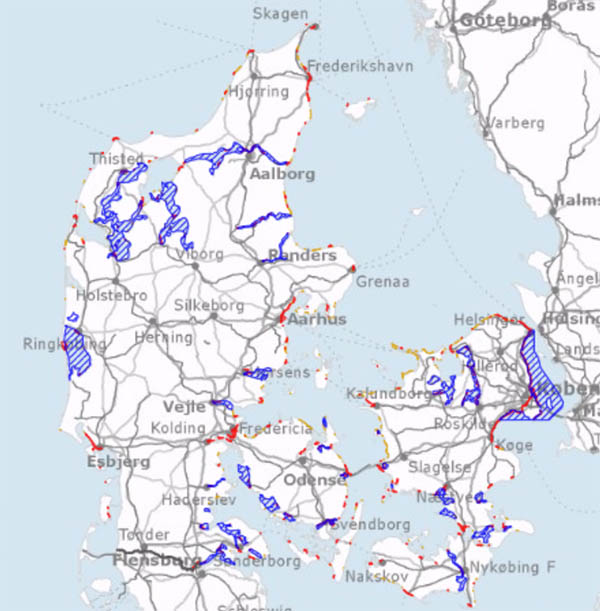
\includegraphics[width=0.45\textwidth]{Billeder/Andet/reservatkort.jpg}
        % Eller: [height=0.6\textheight] for højde-baseret skalering
    \end{center}
    
    % Her kan du tilføje tekst under billedet
    \vspace{1em}
    
\end{frame}

\begin{frame}{Jagt på fiskeriterritoriet – is og særlige begrænsninger (§7)}
    \begin{itemize}
        \item \textbf{§7 stk. 1}: På fiskeriterritoriet må der \textbf{ikke} drives jagt
          \begin{itemize}
            \item Fra is
            \item Inden for 100 m fra iskant
          \end{itemize}
        \item \textbf{Stk. 2}: Reglen i stk. 1 gælder \textbf{ikke} for jagt på \textbf{ræv}
    \end{itemize}
\end{frame}



\begin{frame}{Jagt fra båd – forbud og begrænsninger (§8)}
    \begin{itemize}
        \item \textbf{§8 stk. 1}: Der må \textbf{ikke} drives jagt fra motordrevet fartøj \textbf{i september måned}
        \item \textbf{Stk. 2}: Der må \textbf{ikke} drives jagt fra motordrevet fartøj
          \begin{itemize}
            \item på søer og andre ferske vande
            \item på de dele af fiskeriterritoriet, der er nævnt i \textbf{bilag 1} til bekendtgørelsen (vist på kortbilag)
          \end{itemize}
        \item \textbf{Stk. 3}: Der må \textbf{ikke} sejles med \textbf{ladt} skydevåben på tidspunkter/områder, hvor jagt ikke er tilladt
        \item \textbf{Stk. 4}: Miljøstyrelsen kan i særlige tilfælde dispensere fra stk. 2 (under iagttagelse af habitat- og fuglebeskyttelsesdirektivets artikel 16/9)
    \end{itemize}
\end{frame}

\begin{frame}{Jagt fra båd – hastighedsregler (§9)}
    \begin{itemize}
        \item \textbf{§9}: Til jagt må \textbf{ikke} benyttes motordrevet fartøj, der kan fremføres med mere end \textbf{18 km/t} (ca. 9,7 knob)
        \item Under selve jagtudøvelsen må fartøjet kun fremføres med højst \textbf{5 km/t} (ca. 2,7 knob)
        \item Husk kontekst:
          \begin{itemize}
            \item Generelt forbud mod jagt fra motordrevet fartøj på ferskvand (§26 i jagtloven)
            \item Begrænsede områder på fiskeriterritoriet (bilag 1-kort – ofte kystnære zoner, fjorde mv.)
            \item Ladt våben-forbud gælder uden for tilladte tidspunkter/områder
          \end{itemize}
    \end{itemize}
\end{frame}

\begin{frame}{Jagtmetoder – forbud på fiskeriterritoriet og ferske vande (§10)}
    \begin{itemize}
        \item \textbf{§10}: På fiskeriterritoriet og ferske vande må der \textbf{ikke} jages
          \begin{itemize}
            \item Kronvildt
            \item Dåvildt
            \item Sikavildt
            \item Råvildt
            \item Harer
            \item Mufloner
            \item Vildsvin
          \end{itemize}
        \item \textbf{Formål}: Beskytte store pattedyr og undgå ulovlig jagt i vandnære områder (supplerer generelle jagttider)
    \end{itemize}
\end{frame}

\begin{frame}{Forbudte hjælpemidler og jagtformer (§11–§12)}
    \begin{itemize}
        \item \textbf{§11}: Til jagt må \textbf{ikke} anvendes
          \begin{itemize}
            \item Mynder eller hunde af mynderacen
            \item Elektronisk udstyr til gengivelse af lyd (elektroniske lokkekald)
            \item Elektronisk udstyr til lokalisering af vildt (varmesøgende/termisk, lysforstærkende/natsigte)
            \item Kunstigt lys, spejle eller andre indretninger til belysning af målet
          \end{itemize}
        \item \textbf{§12}: På kronvildt er \textbf{tryk- og drivjagt} forbudt i perioderne
          \begin{itemize}
            \item 1. september – 15. oktober
            \item 1. februar – 29. februar
          \end{itemize}
        \item \textbf{Definition} (§12 stk. 2): Jagt hvor personer (med/uden hund) bevæger sig rundt og trykker/driver vildtet frem mod posterede skytter
    \end{itemize}
\end{frame}

\begin{frame}{Fodring af kronvildt (§13)}
    \begin{itemize}
        \item \textbf{§13 stk. 1}: Kronvildt må \textbf{ikke} fodres med valset korn eller kraftfoder
        \item \textbf{Stk. 2}: Øvrig fodring af kronvildt skal ske i mindst \textbf{130 m} afstand fra
          \begin{itemize}
            \item Platforme og skydestiger (jf. §1 stk. 2)
            \item Anden ejendom
          \end{itemize}
        \item \textbf{Stk. 3} – Undtagelse: Fodring nærmere end 130 m fra anden ejendom tilladt på ejendomme, hvor ejeren \textbf{ikke} har overdraget jagtretten på kronvildt til andre
        \item Husk: Generelt forbud mod udfodring med jagt for øje (§28 i bekendtgørelsen)
    \end{itemize}
\end{frame}

\section{Jagtformer}

\begin{frame}
  \vspace{3em}
  \begin{center}
    {\LARGE \textbf{Jagtformer}
    }
    \\
    \vspace{1em}
  \end{center}
\end{frame}


\begin{frame}{Pürsch}
    
    \begin{columns}[T]
        \begin{column}{0.58\textwidth}
            \begin{itemize}
                \item Jægeren opsøger vildtet \textbf{aktivt} i terrænet
                \item Bevægelse foregår \textbf{langsomt} og lydløst (ofte mod vinden)
                \item Stor vægt på \textbf{opsøgende evner} og viden om dyrets adfærd
                \item Ingen drivere eller standpladser
                \item Klassisk form for storvildtjagt (rådyr, kronvildt, dåvildt)
                \item Kræver god kondition og tålmodighed
                \item Der anvendes ikke hund til denne jagtform
                \item Der anvendes riffel, bue (ikke haglgevær)
            \end{itemize}
        \end{column}
        
        \begin{column}{0.4\textwidth}
            \centering
            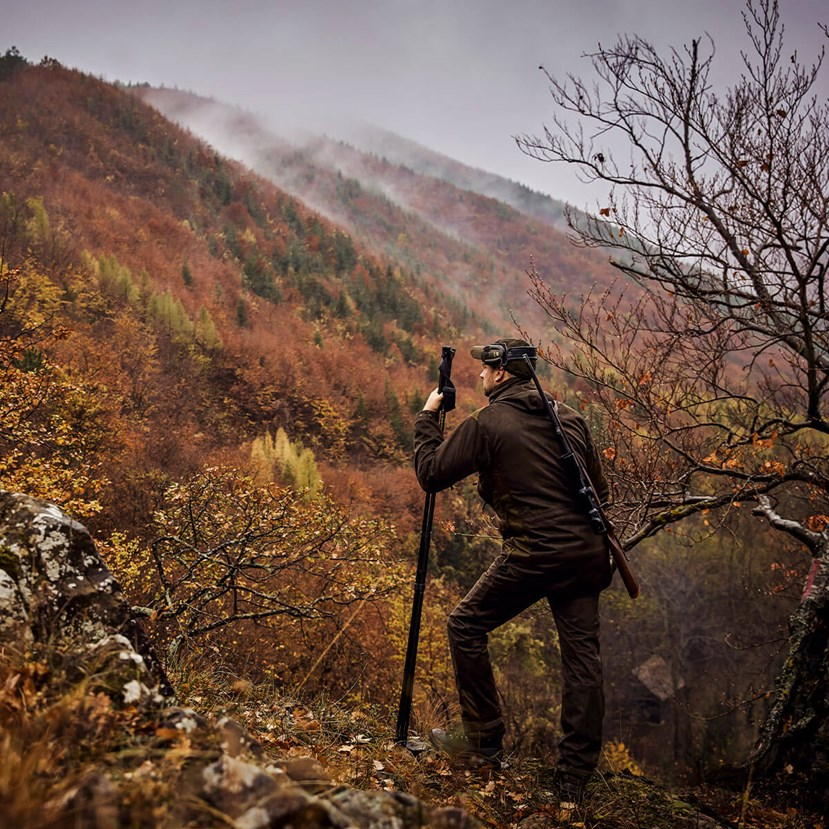
\includegraphics[width=\textwidth,height=0.85\textheight,keepaspectratio]
                {Billeder/Jagtformer/pursch}
            % Alternativt brug en af disse stilrene billeder:
            % \includegraphics[width=\textwidth]{highseat-snow-forest-hunter.jpg}
            % \includegraphics[width=\textwidth]{hunter-leaning-tree-rifle.jpg}
        \end{column}
    \end{columns}
    
\end{frame}


\begin{frame}{Trampejagt}
    
    \begin{columns}[T]
        \begin{column}{0.58\textwidth}
            \begin{itemize}
                \item Aktiv jagtform med mange deltagere
                \item Klassisk social og gammeldags jagtform
                \item Arealer drives af med jægere og drivere i tæt drev
                \item Der er ikke for- og bagposter placeret
                \item Der anvedes hunde med kort søg
                \item Der anvendes haglgevær
            \end{itemize}
        \end{column}
        
        \begin{column}{0.4\textwidth}
            \centering
            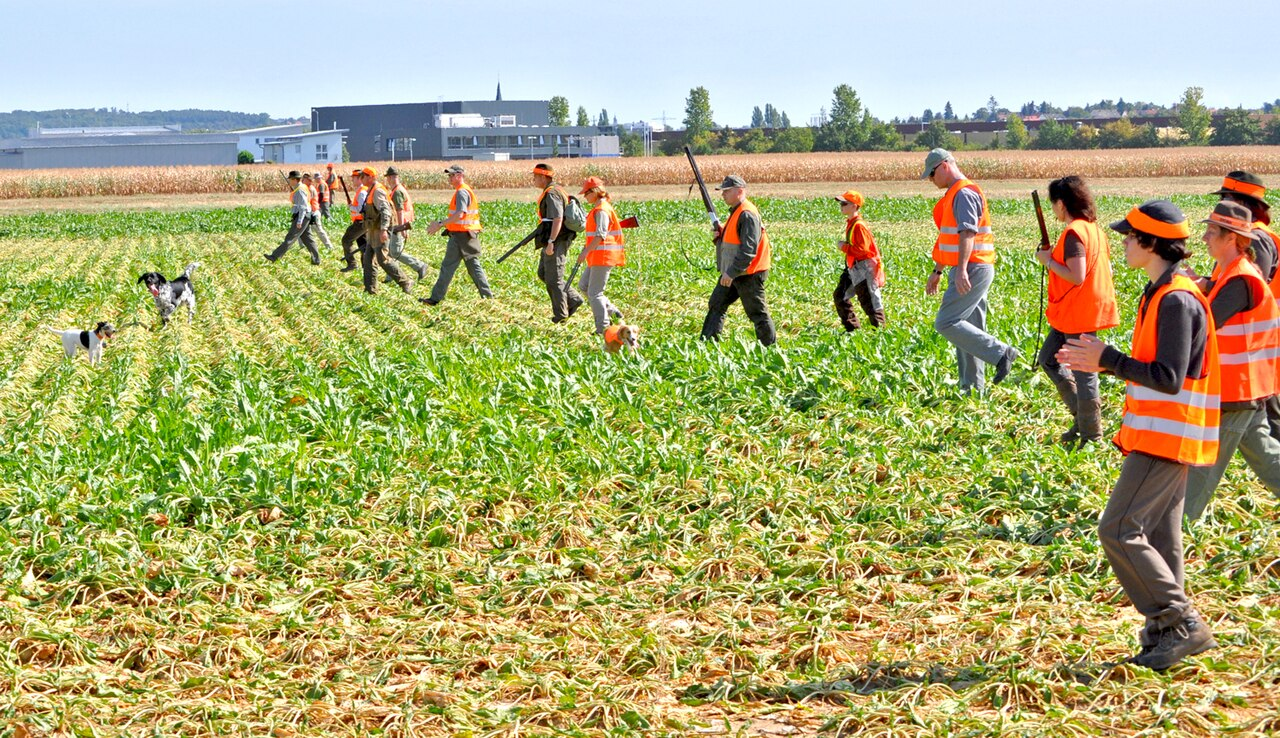
\includegraphics[width=\textwidth,height=0.85\textheight,keepaspectratio]
                {Billeder/Jagtformer/trampejagt_01}
            % Alternativt brug en af disse stilrene billeder:
            % \includegraphics[width=\textwidth]{highseat-snow-forest-hunter.jpg}
            % \includegraphics[width=\textwidth]{hunter-leaning-tree-rifle.jpg}
        \end{column}
    \end{columns}
    
\end{frame}


\begin{frame}{Trykjagt (bewegungsjagt)}
    
    \begin{columns}[T]
        \begin{column}{0.58\textwidth}
            \begin{itemize}
                \item Semi-aktiv jagtform med få drivere 
                \item Jægere placeres vilkårligt i terræn
                \item Få drivere skubber rundt til hovdyr
                \item Der anvendes riffel eller bue
                \item Der anvendes sjældent hunde i så fald meget kortsøgende eller i snor
                \item Dyrene kommer langsomt (=bedre skydning/afskydning))
                \item Jægere er typisk placeret i stiger, tårne eller treestand
            \end{itemize}
        \end{column}
        
        \begin{column}{0.4\textwidth}
            \centering
            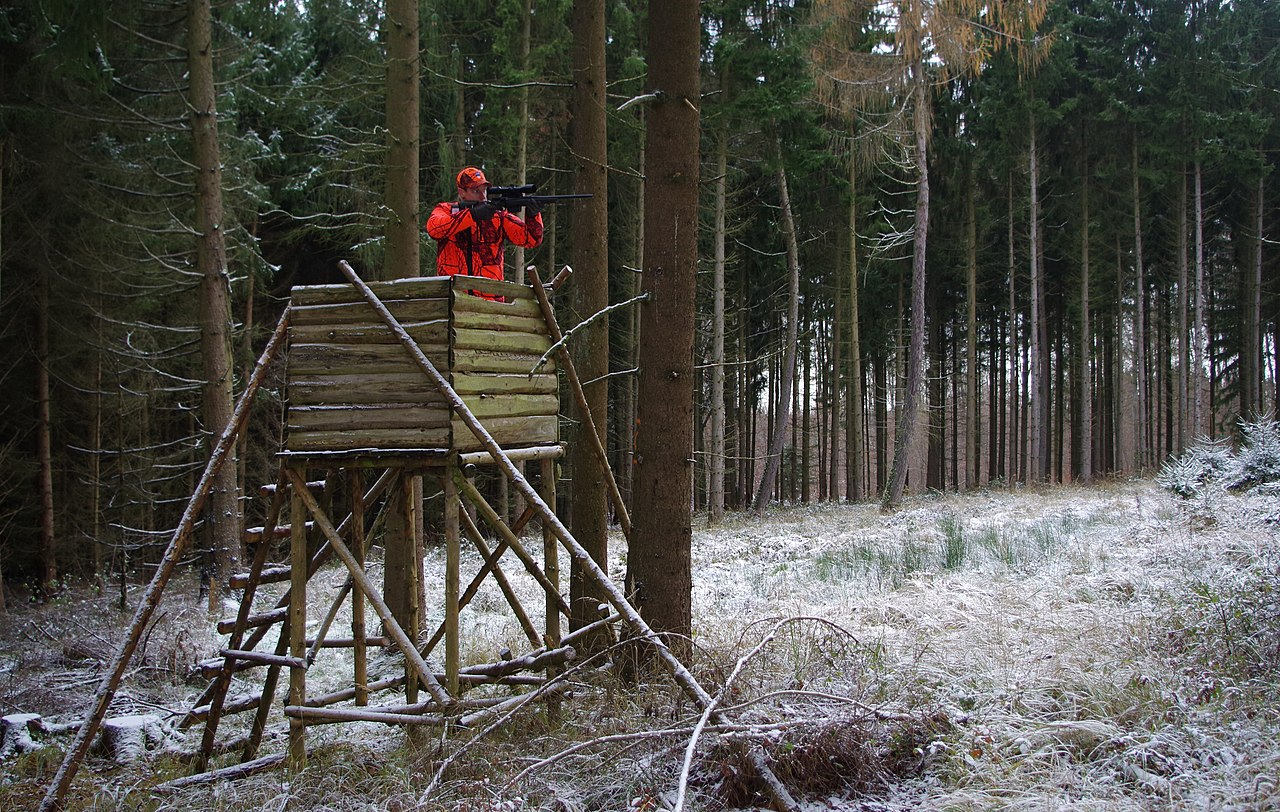
\includegraphics[width=\textwidth,height=0.85\textheight,keepaspectratio]
                {Billeder/Jagtformer/trykjagt_01}
            % Alternativt brug en af disse stilrene billeder:
            % \includegraphics[width=\textwidth]{highseat-snow-forest-hunter.jpg}
            % \includegraphics[width=\textwidth]{hunter-leaning-tree-rifle.jpg}
        \end{column}
    \end{columns}
    
\end{frame}

\begin{frame}{Drivjagt}
    
     \begin{columns}[T]
        \begin{column}{0.58\textwidth}
            \begin{itemize}
                \item \textbf{Semi-aktiv} jagtform – vildtet drives frem til jægerne
                \item Jægeren placeres rundt om området der drives
                \item Jægeren er typisk placeret i jagttårn el lign
                \item Vildtet kommer hurtigt
                \item Større krav til skydefærdigheder
                \item Alle våbentyper i brug
                \item Tæt systematisk drev (drevet går på linie)
                \item Anvendeligt på meget store arealer
                \item Anvendes langsomme jagthunde (terrier, beagle etc)
            \end{itemize}
        \end{column}
        
         \begin{column}{0.4\textwidth}
            \centering
            \vspace{0.5em}
            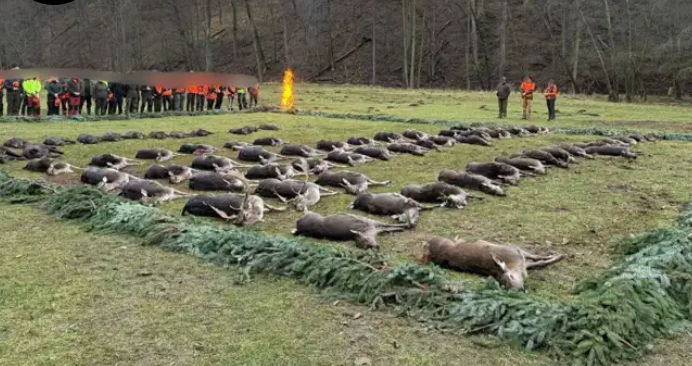
\includegraphics[width=\textwidth,height=0.82\textheight,keepaspectratio]
                {Billeder/Jagtformer/drivjagt}
            % Alternativer – fjern kommentartegn hvis du vil skifte:
            % \includegraphics[width=\textwidth]{highseat-snow-forest-hunter.jpg}
            % \includegraphics[width=\textwidth]{hunter-highseat-morning-mist.jpg}
            % \includegraphics[width=\textwidth]{ansitz-jagttarn-skov.jpg}
        \end{column}
    \end{columns}
    
\end{frame}

\begin{frame}{Anstandsjagt}
    
     \begin{columns}[T]
        \begin{column}{0.58\textwidth}
            \begin{itemize}
                \item \textbf{Passiv} jagtform – jægeren venter på vildtet
                \item Jægeren placerer sig strategisk i terrænet
                \item Foregår typisk fra: jagttårn, jagtstige, treestand
                \item Fordele:
                  \begin{itemize}
                    \item Kontrolleret og sikkert skud
                    \item God styr på vindretning
                    \item Vildtet forstyrres minimalt
                  \end{itemize}
                \item Vildtet drives ikke frem – det kommer naturligt
                \item Meget udbredt på hjortevildt (råvildt, dåvildt, kronvildt)
                \item Kræver tålmodighed, god placering og viden om vildtets færden
                \item Anvendes ikke hunde til denne jagtform
            \end{itemize}
        \end{column}
        
         \begin{column}{0.4\textwidth}
            \centering
            \vspace{0.5em}
            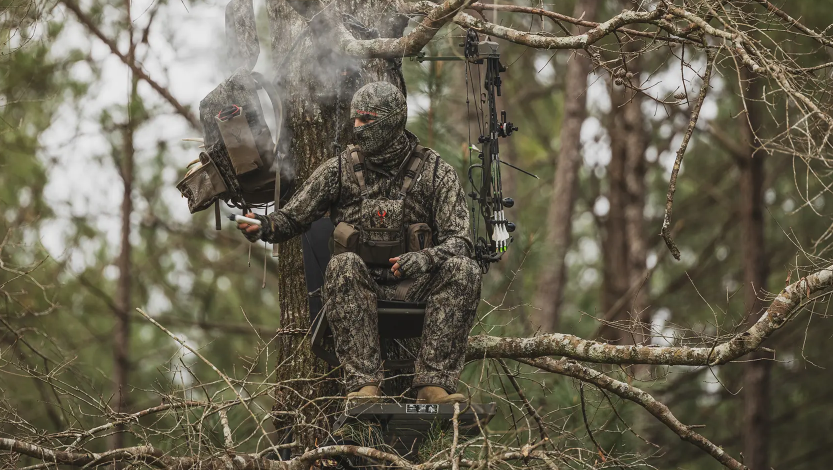
\includegraphics[width=\textwidth,height=0.82\textheight,keepaspectratio]
                {Billeder/Jagtformer/anstandsjagt.png}
            % Alternativer – fjern kommentartegn hvis du vil skifte:
            % \includegraphics[width=\textwidth]{highseat-snow-forest-hunter.jpg}
            % \includegraphics[width=\textwidth]{hunter-highseat-morning-mist.jpg}
            % \includegraphics[width=\textwidth]{ansitz-jagttarn-skov.jpg}
        \end{column}
    \end{columns}
    
\end{frame}


\begin{frame}{Trækjagt}
    
    \begin{columns}[T]
        \begin{column}{0.58\textwidth}
            \begin{itemize}
                \item Passiv jagtform - venter på trækkende fugle
                \item Solo eller få jægere sammen
                \item Der anvendes skjul, camouflage og lokkefugle
                \item Meget udbredt jagtform i DK
                \item Der anvendes haglgevær
                \item Der anvendes apporterende hunde (lovkrav)
            \end{itemize}
        \end{column}
        
        \begin{column}{0.4\textwidth}
            \centering
            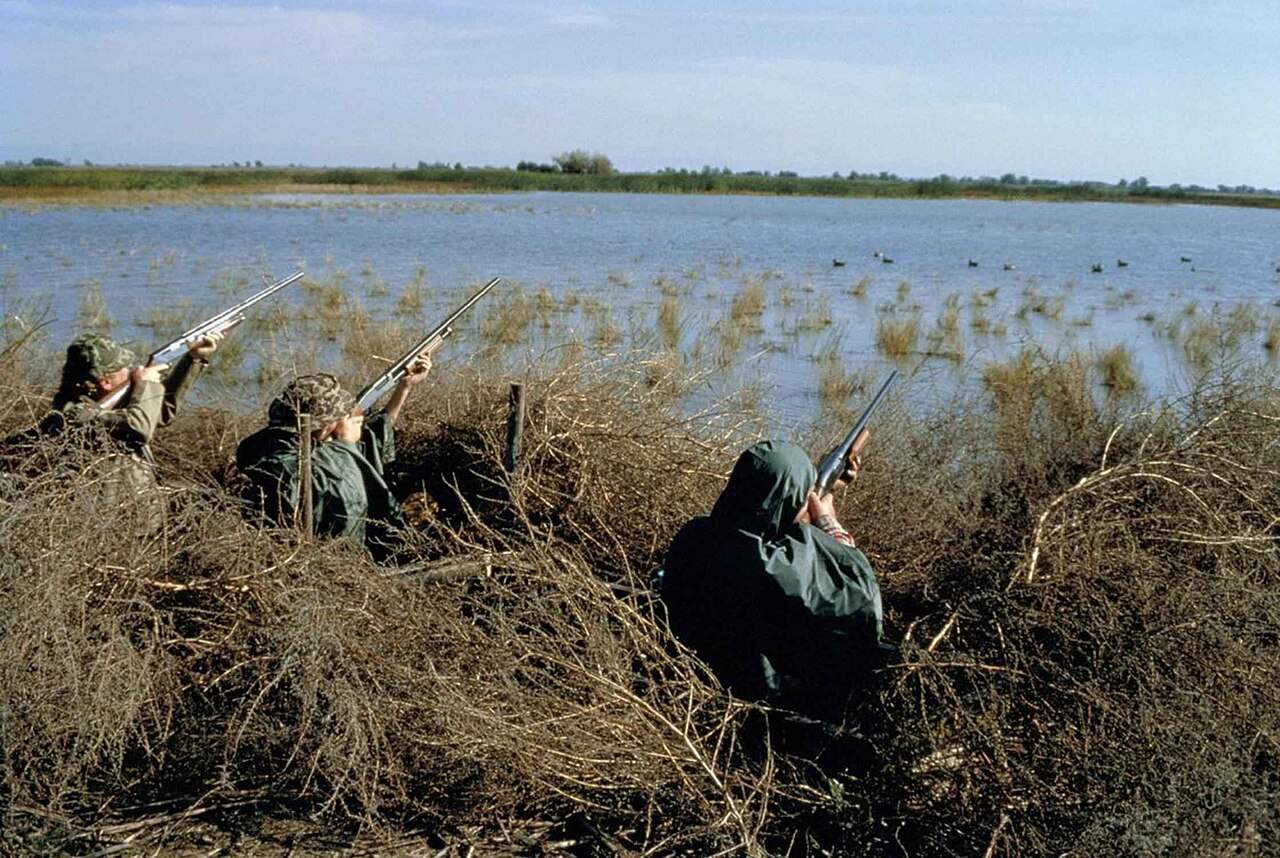
\includegraphics[width=\textwidth,height=0.85\textheight,keepaspectratio]
                {Billeder/Jagtformer/traekjagt_01}
            % Alternativt brug en af disse stilrene billeder:
            % \includegraphics[width=\textwidth]{highseat-snow-forest-hunter.jpg}
            % \includegraphics[width=\textwidth]{hunter-leaning-tree-rifle.jpg}
        \end{column}
    \end{columns}
    
\end{frame}


\begin{frame}{Strand- og havjagt}
    
    \begin{columns}[T]
        \begin{column}{0.58\textwidth}
            \begin{itemize}
                \item Pramjagt (passiv) - venter på trækkende fugle
                \item Motorbådsjagt (aktiv) - sejler med vinden mod fuglene
                \item Max hastighed 5 km/t under jagt
                \item Max hastighed 18 km/t før/efter jagt
                \item Gratis på fiskeriterritoriet
                \item Vær påpasselig med vejr, udstyr og sikkerhed
                \item Haglgevær anvendes
                \item Der anvendes typisk ikke hunde til jagtformen
            \end{itemize}
        \end{column}
        
        \begin{column}{0.4\textwidth}
            \centering
            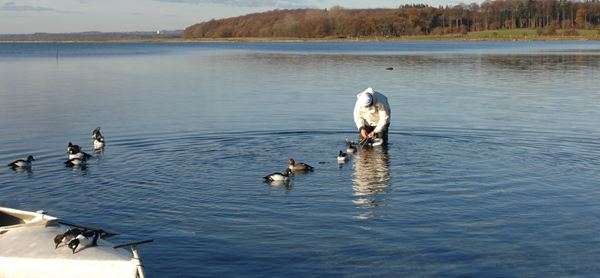
\includegraphics[width=\textwidth,height=0.85\textheight,keepaspectratio]
                {Billeder/Jagtformer/havjagt}
            % Alternativt brug en af disse stilrene billeder:
            % \includegraphics[width=\textwidth]{highseat-snow-forest-hunter.jpg}
            % \includegraphics[width=\textwidth]{hunter-leaning-tree-rifle.jpg}
        \end{column}
    \end{columns}
    
\end{frame}

\begin{frame}{Jagt for stående hund}
    
     \begin{columns}[T]
        \begin{column}{0.58\textwidth}
            \begin{itemize}
                \item \textbf{Aktiv} jagtform – hund med stort søg står stand ved typisk hønsefugl
                \item Typisk solo eller få jægere
                \item Jægeren giver signal til hunden om at lette fuglen ved stand
                \item Der anvendes glatløbet haglgevær til jagtformen
                \item Uddøende jagtform i DK pga. den intensive arealudnyttelse
            \end{itemize}
        \end{column}
        
         \begin{column}{0.4\textwidth}
            \centering
            \vspace{0.5em}
            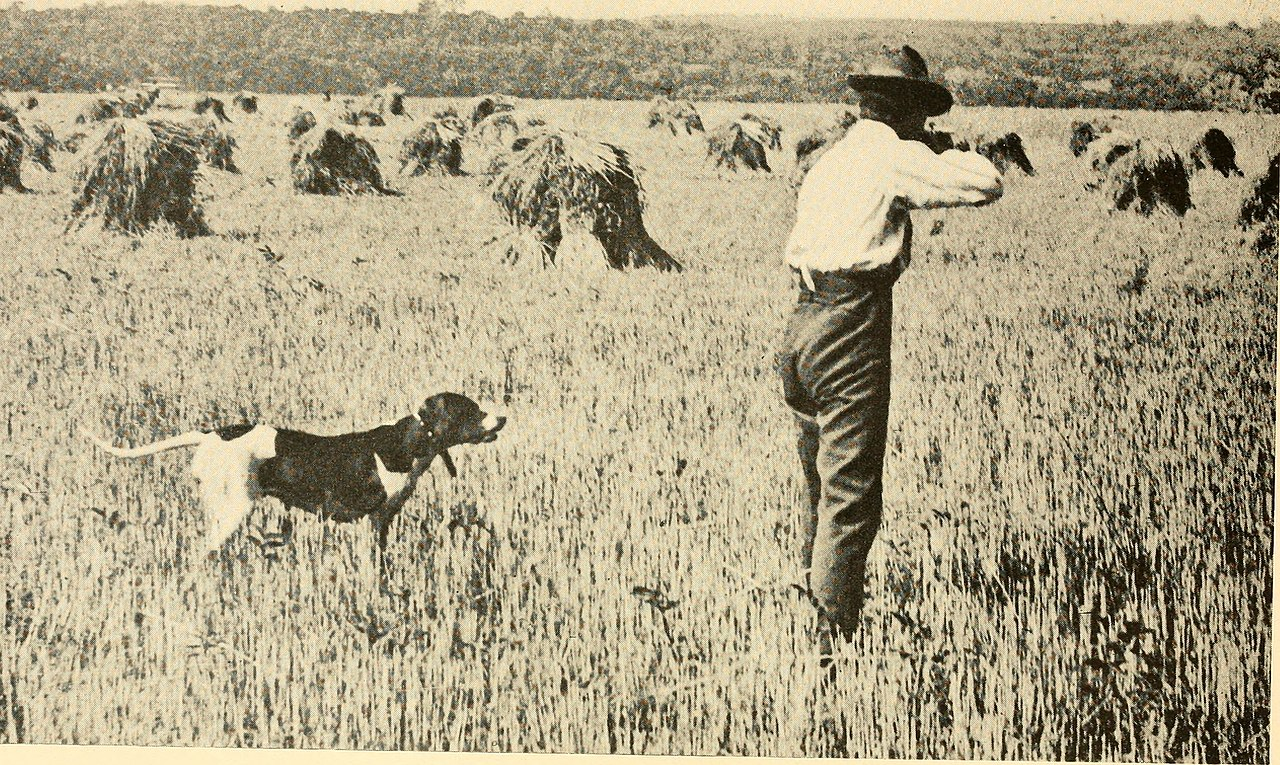
\includegraphics[width=\textwidth,height=0.82\textheight,keepaspectratio]
                {Billeder/Jagtformer/staaende_jagt}
            % Alternativer – fjern kommentartegn hvis du vil skifte:
            % \includegraphics[width=\textwidth]{highseat-snow-forest-hunter.jpg}
            % \includegraphics[width=\textwidth]{hunter-highseat-morning-mist.jpg}
            % \includegraphics[width=\textwidth]{ansitz-jagttarn-skov.jpg}
        \end{column}
    \end{columns}
    
\end{frame}





\begin{frame}{Jagt for stødende hund (rough shooting)}
    
     \begin{columns}[T]
        \begin{column}{0.58\textwidth}
            \begin{itemize}
                \item \textbf{Aktiv} jagtform – hund med kort søg letter vildtet som typisk nedlægges i bagskud 
                \item Typisk solo eller få jægere
                \item Der anvendes glatløbet haglgevær til jagtformen
                \item Udbredt jagtform i DK - passer til små arealer
            \end{itemize}
        \end{column}
        
         \begin{column}{0.4\textwidth}
            \centering
            \vspace{0.5em}
            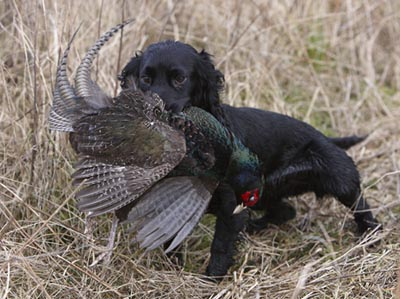
\includegraphics[width=\textwidth,height=0.82\textheight,keepaspectratio]
                {Billeder/Jagtformer/stoedende_01}
            % Alternativer – fjern kommentartegn hvis du vil skifte:
            % \includegraphics[width=\textwidth]{highseat-snow-forest-hunter.jpg}
            % \includegraphics[width=\textwidth]{hunter-highseat-morning-mist.jpg}
            % \includegraphics[width=\textwidth]{ansitz-jagttarn-skov.jpg}
        \end{column}
    \end{columns}
    
\end{frame}

\begin{frame}{Gravjagt}
    
     \begin{columns}[T]
        \begin{column}{0.58\textwidth}
            \begin{itemize}
                \item \textbf{Aktiv} jagtform – ræv jages ud af graven med gravsøgende hunde
                \item Jægerne placerer sig ved udgangene til gravsystemet
                \item Der anvendes glatløbet haglgevær til jagtformen
                \item Frivillige certificeringer af egnede hunde (gravhund/jack russell o.lign)
            \end{itemize}
        \end{column}
        
         \begin{column}{0.4\textwidth}
            \centering
            \vspace{0.5em}
            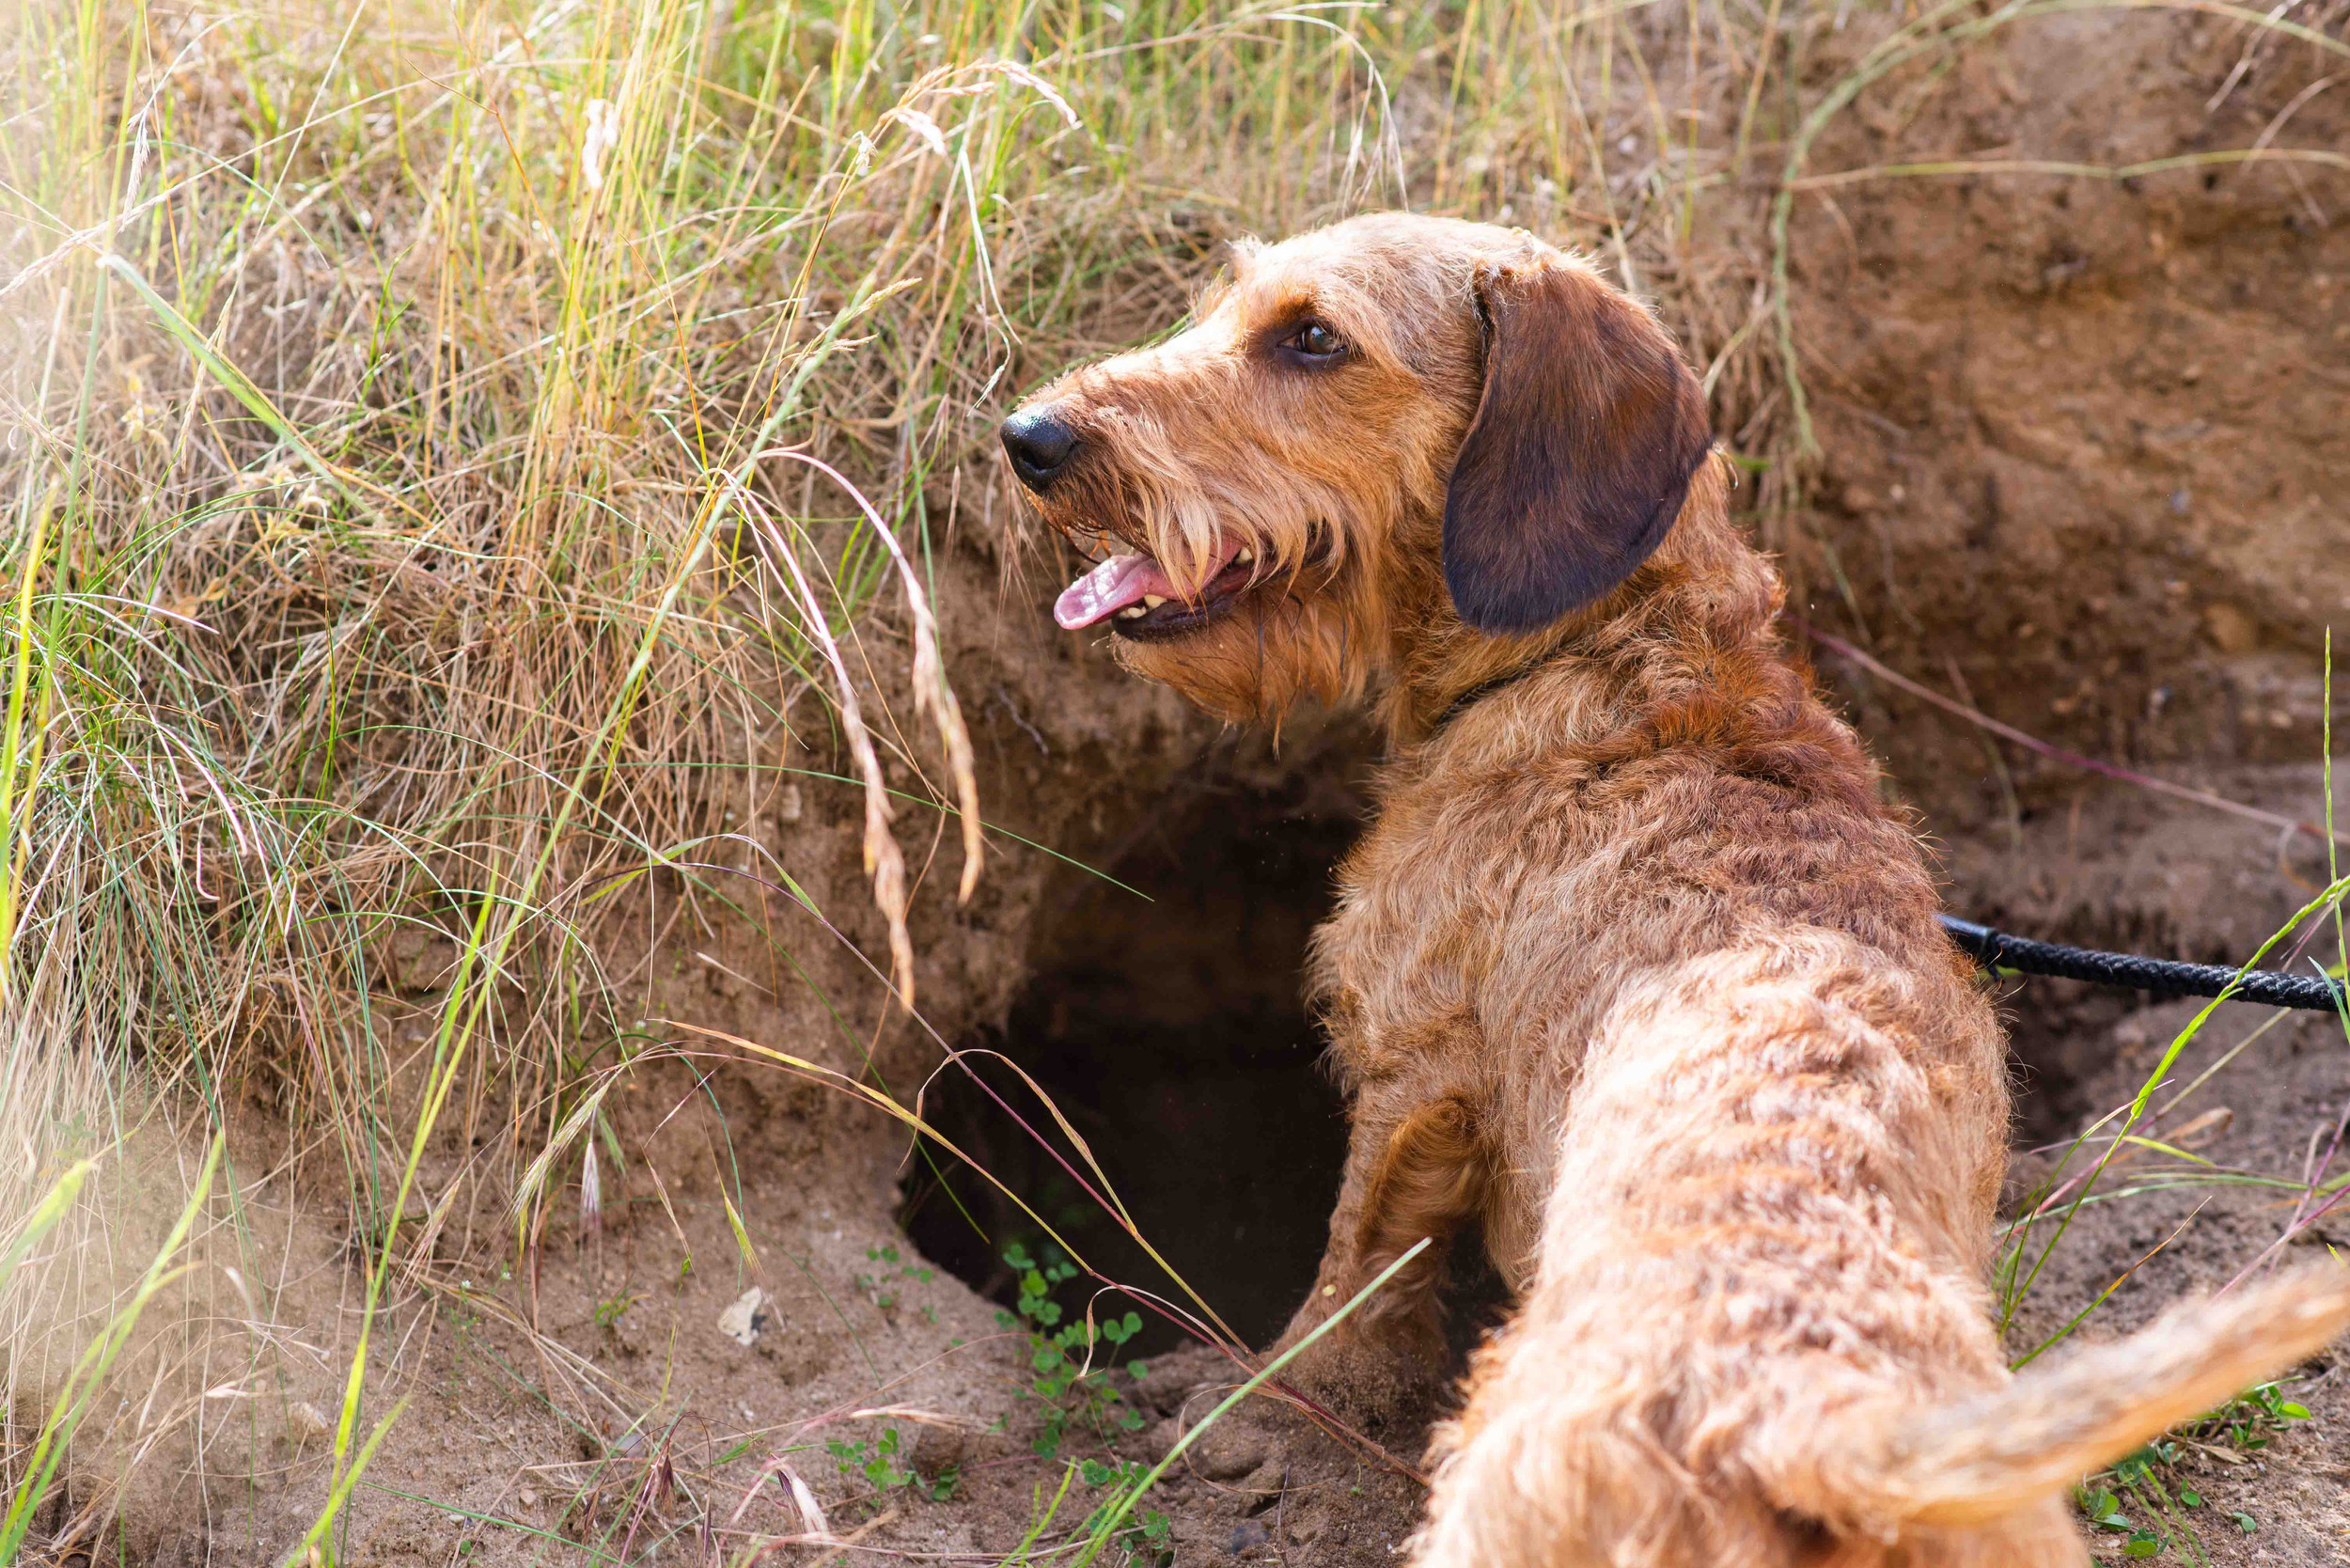
\includegraphics[width=\textwidth,height=0.82\textheight,keepaspectratio]
                {Billeder/Jagtformer/gravjagt}
            % Alternativer – fjern kommentartegn hvis du vil skifte:
            % \includegraphics[width=\textwidth]{highseat-snow-forest-hunter.jpg}
            % \includegraphics[width=\textwidth]{hunter-highseat-morning-mist.jpg}
            % \includegraphics[width=\textwidth]{ansitz-jagttarn-skov.jpg}
        \end{column}
    \end{columns}
    
\end{frame}

\section{Jagthunde}

\begin{frame}
  \vspace{3em}
  \begin{center}
    {\LARGE \textbf{Jagthunde}
    }
    \\
    \vspace{1em}
  \end{center}
\end{frame}

\begin{frame}{Bekendtgørelse af lov om jagt og vildtforvaltning § 24} % Lige justering af titlen
\vspace{1em}
\begin{columns}[c] % c = center vertically
\column{0.05\textwidth} % Venstre margin
\column{0.7\textwidth} % Midten: Bullets
\small
\raggedright
\begin{itemize}
\itemsep0.6em % Justér afstand mellem bullets
\item § 24. Ved jagt med glatløbet haglgevær på ikkeklovbærende vildt på og fra landarealer og i rør- og sivbevoksninger skal egnet apporterende hund medbringes.
\end{itemize}
\column{0.25\textwidth} % Højre: Ikon
\centering
\vspace{0pt}
% Der skal formentlig indsættes et passende billede/ikon her
\end{columns}
\end{frame}

\begin{frame}{Overordnede kategorier af jagthunde}

\vspace{1em}

\begin{columns}[c] % c = center vertically

\column{0.05\textwidth} % Venstre margin

\column{0.7\textwidth} % Midten: Bullets

\small

\raggedright

\begin{itemize}

\itemsep0.6em % Justér afstand mellem bullets

\item \textbf{Stående} (f.eks. Irsk Setter)
\item \textbf{Stødende} (f.eks. Cocker Spaniel)
\item \textbf{Apporterende} (f.eks. Labrador, Golden Retriever)
\item \textbf{Gravsøgende} (f.eks. Gravhund)
\item \textbf{Støvende (drivende)} (f.eks. Beagle)
\item \textbf{Schweisshunde} (f.eks. Blodhund)

\end{itemize}

\column{0.25\textwidth} % Højre: Ikon

\centering

\vspace{0pt}

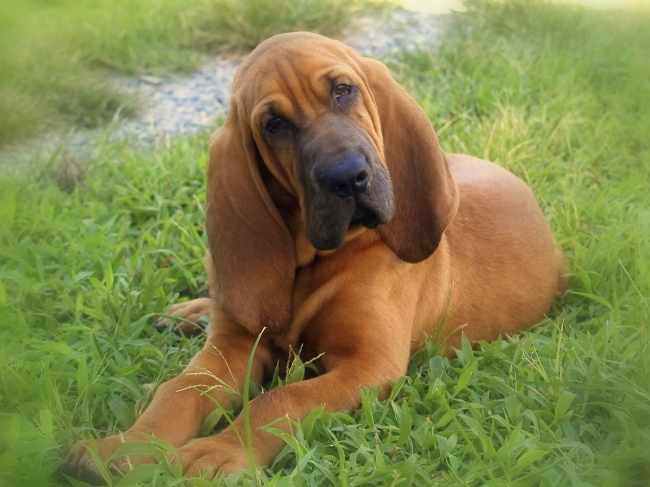
\includegraphics[width=0.9\linewidth]{Billeder/Jagthunde/schweisshunde/blodhund.jpg} % Ændret ikon til at passe med 'Hunde'

\end{columns}

\end{frame}

\begin{frame}{Apporterende jagthunde}

\vspace{1em}

\begin{columns}[c] % c = center vertically

\column{0.05\textwidth} % Venstre margin

\column{0.7\textwidth} % Midten: Bullets

\small

\raggedright

\begin{itemize}

\itemsep0.6em % Justér afstand mellem bullets

\item Hovedopgaven er at \textbf{finde og bringe nedlagt vildt} til jægeren (apportere).
\item Skal være \textbf{skudfast} og have en \textbf{blød mund} for ikke at ødelægge vildtet.
\item Er nødvendig ved jagt med haglgevær på ikke-klovbærende vildt på landarealer (§ 24).
\item Er ofte velegnede \textbf{familiehunde} grundet deres samarbejdsvilje.
\item \textbf{Racer}: Labrador Retriever, Golden Retriever, Flatcoated Retriever, Chesapeake Bay Retriever.

\end{itemize}

\column{0.25\textwidth} % Højre: Ikon

\centering

\vspace{0pt}

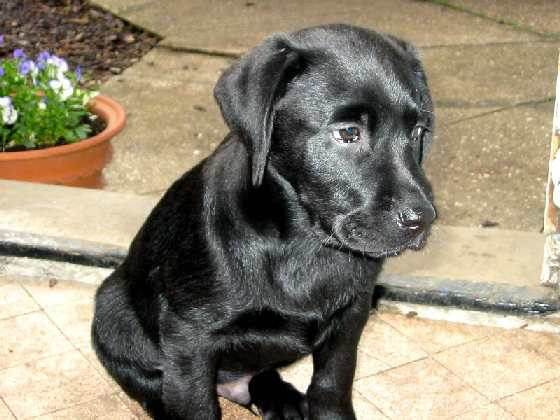
\includegraphics[width=0.9\linewidth]{Billeder/Jagthunde/apporterende/labrador.jpg} % Ikon af apporterende hund

\end{columns}

\end{frame}

\begin{frame}{Stødende jagthunde}

\vspace{1em}

\begin{columns}[c] % c = center vertically

\column{0.05\textwidth} % Venstre margin

\column{0.7\textwidth} % Midten: Bullets

\small

\raggedright

\begin{itemize}

\itemsep0.6em % Justér afstand mellem bullets

\item Hundens opgave er at \textbf{søge under bøssen} (tæt på jægeren) og rejse vildtet.
\item De skal "støde" vildtet, dvs. få det til at \textbf{flyve eller løbe op} inden for skudafstand.
\item Har typisk en \textbf{kort rækkevidde} i søget og arbejder tæt sammen med jægeren.
\item Bruges primært til jagt på \textbf{fugle} (f.eks. fasaner og ænder) og \textbf{kaniner}.
\item \textbf{Racer}: Cocker Spaniel, Springer Spaniel, Field Spaniel, Kleiner Münsterländer (kan også stå).

\end{itemize}

\column{0.25\textwidth} % Højre: Ikon

\centering

\vspace{0pt}

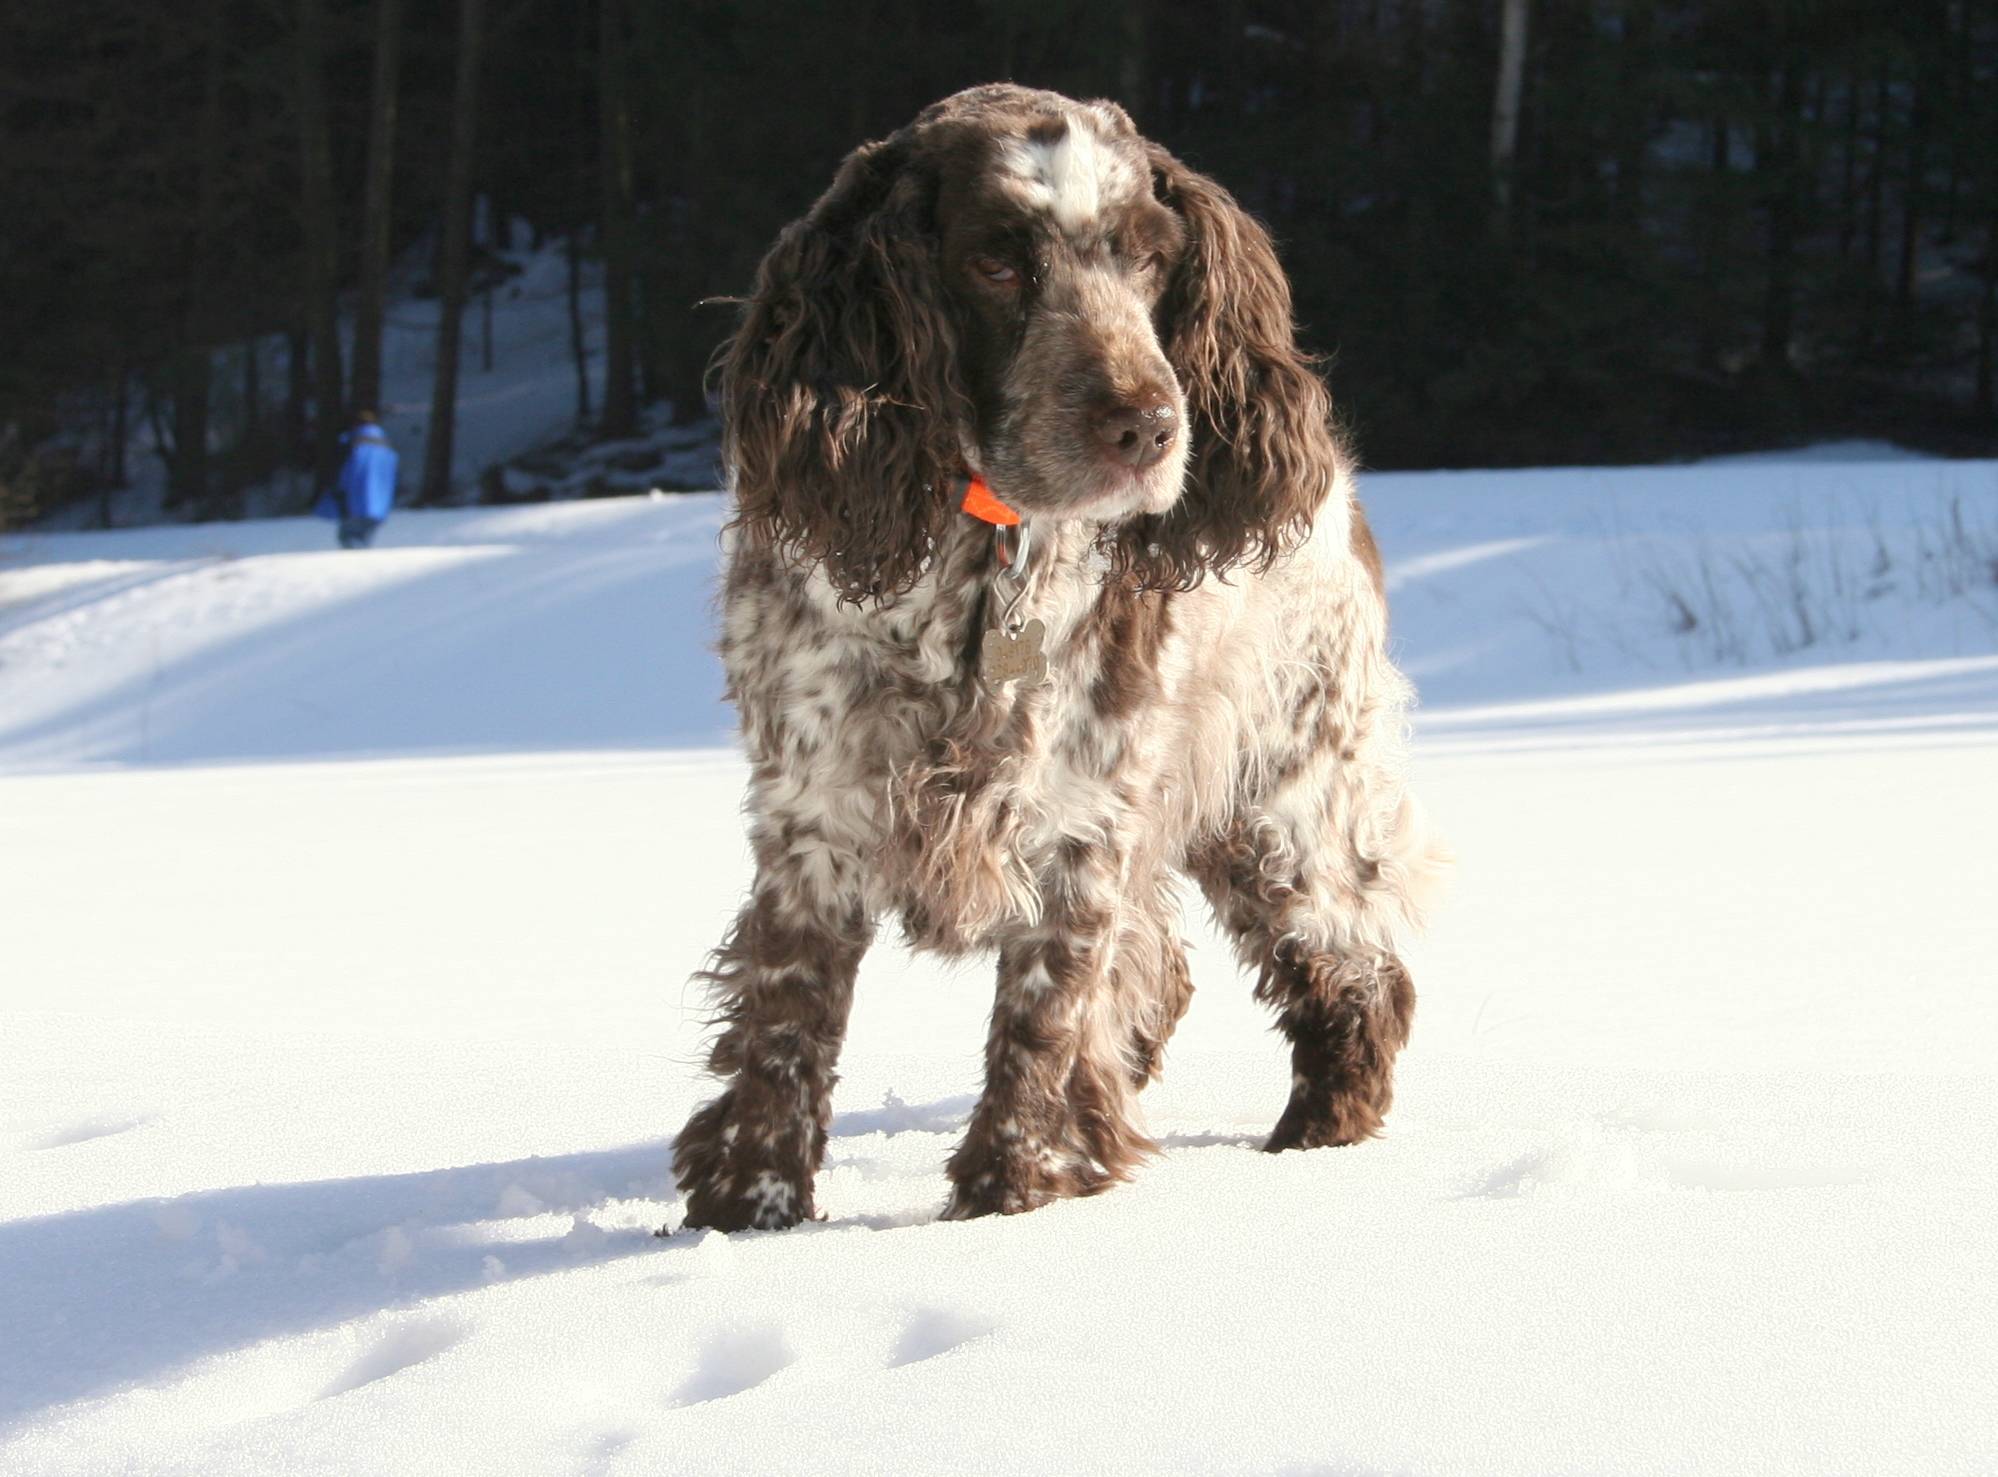
\includegraphics[width=0.9\linewidth]{Billeder/Jagthunde/stoedende/cocker.jpg} % Ikon af en spaniel i aktion

\end{columns}

\end{frame}

\begin{frame}{Stående jagthunde}

\vspace{1em}

\begin{columns}[c] % c = center vertically

\column{0.05\textwidth} % Venstre margin

\column{0.7\textwidth} % Midten: Bullets

\small

\raggedright

\begin{itemize}

\itemsep0.6em % Justér afstand mellem bullets

\item Udfører et \textbf{langt søg} i terrænet.
\item God til jagt i områder med \textbf{stor vildtspredning}.
\item Deres kendetegn er at \textbf{tage stand} for fuglevildt (pege). 
\item Opdeles primært i to typer: \textbf{Engelsk} (f.eks. Pointer, Setter) og \textbf{Kontinental} (f.eks. Ruhåret Hønsehund).
\item Anvendes til jagt på hønsefugle - jagtformen er aftagende.
\item \textbf{Racer}: Hønsehunde, Pointere, Settere, Wizla, Münsterländere, Breton, Weimaraner

\end{itemize}

\column{0.25\textwidth} % Højre: Ikon

\centering

\vspace{0pt}

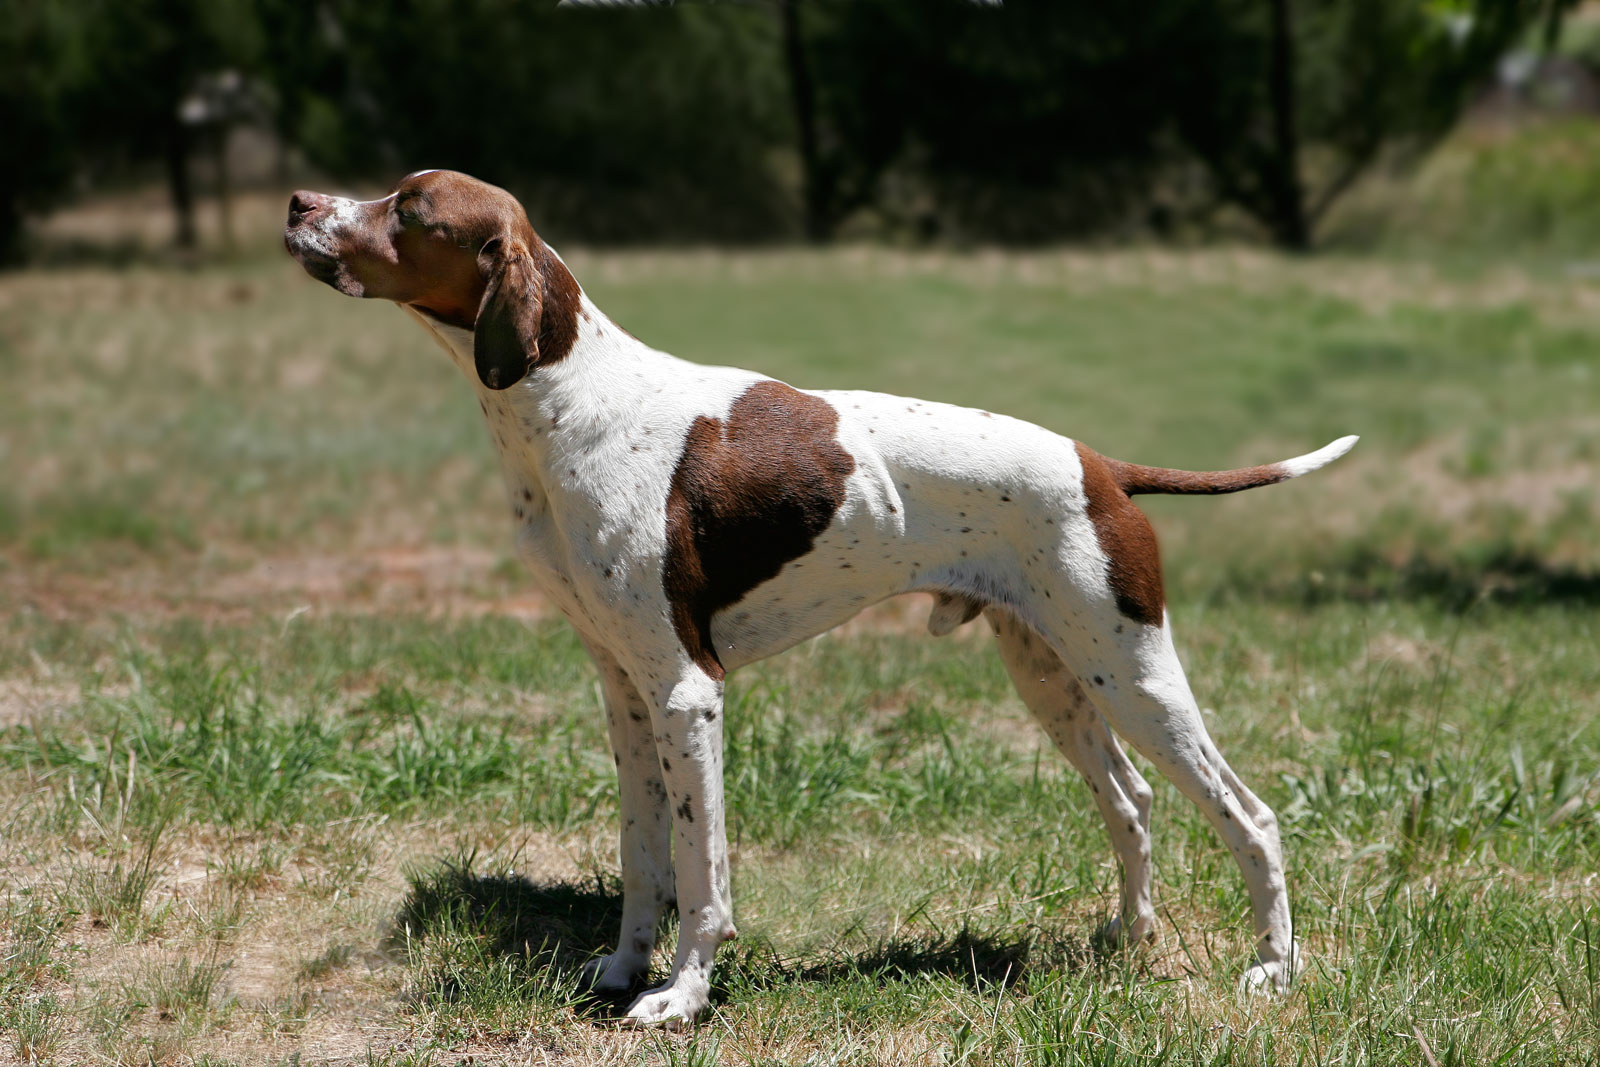
\includegraphics[width=0.9\linewidth]{Billeder/Jagthunde/staaende/English_pointer.jpg} % Ikon af stående hund

\end{columns}

\end{frame}

\begin{frame}{Støvende (Drivende) jagthunde}

\vspace{1em}

\begin{columns}[c] % c = center vertically

\column{0.05\textwidth} % Venstre margin

\column{0.7\textwidth} % Midten: Bullets

\small

\raggedright

\begin{itemize}

\itemsep0.6em % Justér afstand mellem bullets

\item Hundens opgave er at \textbf{støve/drive} vildtet foran sig ved hjælp af gøen og spor.
\item De arbejder \textbf{selvstændigt} og driver vildtet over et stort område mod jægerne (posterne).
\item Brugen er \textbf{stærkt reguleret} i Danmark og må kun anvendes til visse vildtarter.
\item Bruges primært til jagt på \textbf{harer} og \textbf{ridsende klovbærende vildt} (f.eks. råvildt).
\item \textbf{Racer}: Beagle, Basset, Ruhåret Gravhund, de fleste støvere (f.eks. Drever).

\end{itemize}

\column{0.25\textwidth} % Højre: Ikon

\centering

\vspace{0pt}

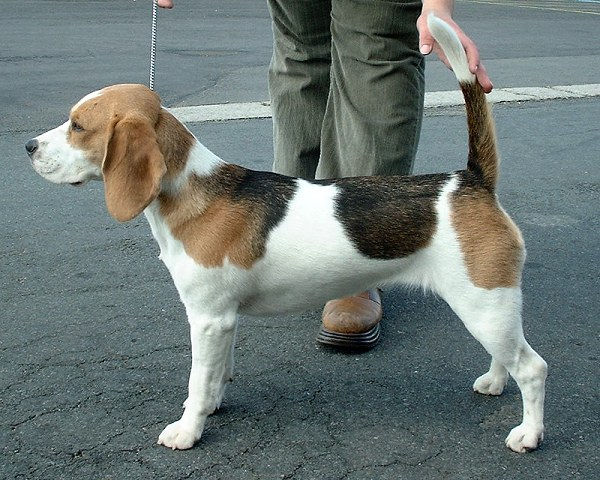
\includegraphics[width=0.9\linewidth]{Billeder/Jagthunde/stoevende/beagle.jpg} % Ikon af en drivende hund (f.eks. Beagle)

\end{columns}

\end{frame}

\begin{frame}{Schweisshunde (Specialister i eftersøgning)}

\vspace{1em}

\begin{columns}[c] % c = center vertically

\column{0.05\textwidth} % Venstre margin

\column{0.7\textwidth} % Midten: Bullets

\small

\raggedright

\begin{itemize}

\itemsep0.6em % Justér afstand mellem bullets

\item Hundens opgave er udelukkende at \textbf{eftersøge anskudt/trafikeret vildt} (Schweiss = blod (tysk)).
\item De arbejder i et spor, der kan være \textbf{flere timer gammelt}, primært i line (sporsele).
\item Enhver jæger har pligt til at \textbf{tilkalde en schweisshundefører}, hvis de anskyder klovbærende vildt.
\item Hundene har en \textbf{trænet lugtesans} og et roligt temperament.
\item \textbf{Racer}: Hannoversk Schweisshund, Bayersk Bjergschweisshund, og i Danmark ofte Ruhåret/Korthåret Hønsehund (som er godkendt til opgaven).

\end{itemize}

\column{0.25\textwidth} % Højre: Ikon

\centering

\vspace{0pt}

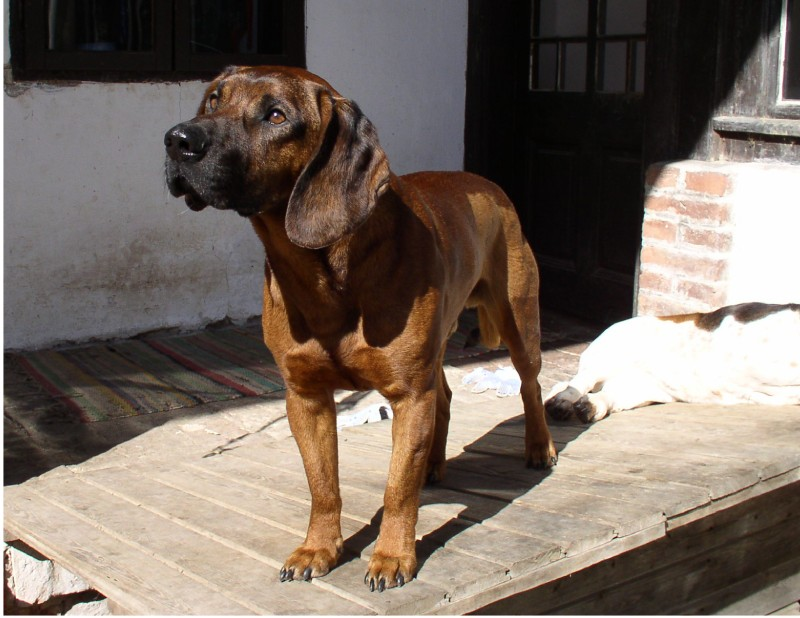
\includegraphics[width=0.9\linewidth]{Billeder/Jagthunde/schweisshunde/schweisshund.jpg} % Ikon af hund i sele/spor

\end{columns}

\end{frame}

\begin{frame}{Gravsøgende jagthunde}

\vspace{1em}

\begin{columns}[c] % c = center vertically

\column{0.05\textwidth} % Venstre margin

\column{0.7\textwidth} % Midten: Bullets

\small

\raggedright

\begin{itemize}

\itemsep0.6em % Justér afstand mellem bullets

\item Hundens opgave er at \textbf{lokalisere og drive vildtet ud af hulen} (gravjagt).
\item Anvendes primært til jagt på \textbf{ræv} i deres huler (grave).
\item Hundene skal have et \textbf{hårdt og modigt sind} og være fysisk rustede til trange miljøer.
\item Gravjagten er en \textbf{særlig jagtform} og er reguleret af Miljøstyrelsen.
\item \textbf{Racer}: Fox Terrier, Jack Russell Terrier, Tysk Jagtterrier, Gravhunde.

\end{itemize}

\column{0.25\textwidth} % Højre: Ikon

\centering

\vspace{0pt}

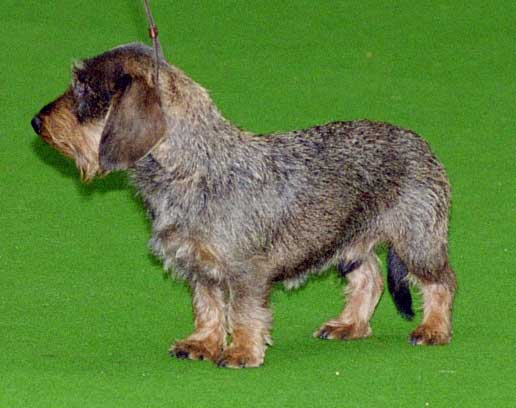
\includegraphics[width=0.9\linewidth]{Billeder/Jagthunde/gravsoegende/gravhund.jpg} % Ikon af gravsøgende hund/gravhund

\end{columns}

\end{frame}

\section{Håndtering af nedlagt vildt}

\begin{frame}
  \vspace{3em}
  \begin{center}
    {\LARGE \textbf{Håndtering af nedlagt vildt}
    }
    \\
    \vspace{1em}
    Hygiejnevejledningen
    \\
    \vspace{1em}
    Vejledning nr. 10099 af 20. december 2023, Kapitel 49
   \end{center}
\end{frame}



\begin{frame}{Affangning af anskudt vildt}
    \begin{itemize}
        \item Mål: Hurtig og smertefri aflivning af anskudt vildt
        \item Fuglevildt: Hårdt slag mod hoved/nakke (træstamme eller stok)
        \item Hare: Slag i nakken eller træk hoved/nakke nedad (hold i bagben)
        \item Rovvildt & større hjortevildt: Ekstra skud (undgå kniv – høj risiko)
        \item Ved brug af hund: Bevar overblik – vent med skud til sikkert
        \item Altid: Prioritér dyrevelfærd og jægersikkerhed
    \end{itemize}
\end{frame}
    

\begin{frame}{Opbrækning af vildt}
    \begin{itemize}
        \item \textbf{Formål}: Fjerne indvolde hurtigt for at undgå gæring, forurening og kødsurhed
        \item Gør det \textbf{straks} efter nedlæggelse (helst inden 30–60 min.)
        \item Grundtrin (klovbærende vildt):
          \begin{itemize}
            \item Læg dyret på ryggen (ben opad) – gerne på rent underlag
            \item Skær fra brystben til hale (åbn bughulen)
            \item Undgå at skære i tarmene/vommen – skær forsigtigt rundt om endetarm
            \item Udtag indvolde samlet (hjerte, lunger, lever, mave, tarme)
            \item Fjern spiserør og luftrør op mod halsen
            \item Tør bughulen ren med klud/papir (ingen vand!)
          \end{itemize}
        \item \textbf{Hygiejne}: Rene hænder/kniv, undgå jord/græs-kontakt
        \item Efter opbrækning: Afkøl hurtigt – hæng op i skygge/køligt sted
        \item https://www.facebook.com/reel/889956353611580
    \end{itemize}
\end{frame}




\begin{frame}{Forlægning af vildt}
    \begin{itemize}
        \item \textbf{Betydning}: Partering/udskæring af klovbærende vildt efter opbrækning
        \item Formål: Adskille kød fra knogler, flå skind af, forberede til modning/konsum
        \item Gøres typisk hjemme eller på jagtstedet efter indvolde er fjernet
        \item Grundtrin (eks. rådyr):
          \begin{itemize}
            \item Hæng dyret op (hoved opad) i køligt sted
            \item Flå skindet af (start ved baglår, træk ned mod hoved)
            \item Fjern hoved, ben og skanker i leddene
            \item Skær ud stykker: stege, culotte, fileter, bov, nakke m.m.
            \item Fjern sener, hinder og fedt efter behov
          \end{itemize}
        \item Hygiejne: Rene redskaber, arbejd køligt, undgå forurening
        \item Modning: Hæng kødet 4–10 dage (afhængig af temperatur (ikke over 7 grader), ca. 40 graddøgn)
    \end{itemize}
\end{frame}
\begin{frame}{Levering til vildthåndteringsvirksomhed – hovedregler}
    \begin{itemize}
        \item Hovedregel: Til vildthåndteringsvirksomhed (samme hygiejne som slagteri)
        \item Nedkøl hurtigt: ≤7 °C storvildt / ≤4 °C småvildt
        \item Luft om dyrene – ingen bunker
        \item Indlever alle dele + organer (undt. gevir/horn/stødtænder; mave/tarme for storvildt)
        \item Uddannet jæger OK → hoved/organer kan udelades (trikiner: altid med for visse arter)
        \item Unormalt: Alle dele med
    \end{itemize}
\end{frame}
\begin{frame}{Direkte afsætning af vildt – forbruger \& lokale butikker}
    \begin{itemize}
        \item Mindre mængder: Direkte til forbruger eller lokale butikker/restauranter
        \item Grænser: 500 småvildt + 15 storvildt pr. år
        \item Organer: Ikke påkrævet med
        \item Trikiner (fx vildsvin): Jæger sørger for undersøgelse
        \item Kontakt Fødevarestyrelsen for lab-info
    \end{itemize}
\end{frame}
\begin{frame}{Vildtdepoter – krav og indretning}
    \begin{itemize}
        \item Registrering: Direkte fra jægere → hos Fødevarestyrelsen
        \item Autorisation: Fra andre depoter
        \item Lager: Ikke nødvendigt inden 12 timer; ellers overdækket, rengørligt, luft om dyr
        \item Nedkøling: Naturlig OK i koldt vejr; aktiv ved sommer/lang tid
        \item Temperatur: ≤7 °C storvildt / ≤4 °C småvildt
        \item Undgå bunker for bedre afkøling
    \end{itemize}
\end{frame}
\begin{frame}{Primærproducenter vs. konsortier \& lodsejere}
    \begin{itemize}
        \item Enkelt jæger: Primærproducent → direkte salg til forbruger OK
        \item Konsortium som helhed / lodsejer: Ikke primærproducent → ingen direkte salg
        \item Løsning: Registrer som vildtdepot → levering til vildthåndteringsvirksomhed
        \item Direkte til forbruger: Via registreret detailudsalg
        \item Jagtparade: Salg til deltagere uden registrering (kun egen husholdning)
    \end{itemize}
\end{frame}
\begin{frame}{Uddannelse – krav til jægere ved markedsføring}
    \begin{itemize}
        \item Kendskab til: Vildtpatologi, håndtering af vildt \& kød
        \item Tilstrækkeligt: Én uddannet person pr. jagtselskab/konsortium
        \item Selskabet sikrer kravet opfyldes
        \item Kursus: Vildtsygdomme \& hygiejne (DJ m.fl.)
    \end{itemize}
\end{frame}
\begin{frame}{Vurdering af vildt (§49.6)}
    \begin{itemize}
        \item \textbf{Hovedregel}: Vildt/kød skal vurderes af \textbf{uddannet person} (se §49.5)
        \item \textbf{Undtagelse}: Ikke krav ved direkte levering til endelig forbruger eller lokale detailbutikker (restauranter, vildtbutikker, supermarkeder)
        \item \textbf{Vurderingens indhold}:
          \begin{itemize}
            \item Adfærd før nedlæggelse (observeret af uddannet person eller beskrevet af nedlæggeren)
            \item Krop og organer efter nedlæggelse (tegn på sygdom, forurening m.m.)
          \end{itemize}
        \item \textbf{Jægererklæring} (kun storvildt til vildthåndteringsvirksomhed):
          \begin{itemize}
            \item Udstedes af uddannet person
            \item Indeholder: Dato, tid, sted for nedlæggelse; navn, underskrift, evt. jagttegnsnummer
            \item Kan dække flere dyr (med identifikationsnumre)
            \item To standarder: Normal (alt OK) eller unormal (problemer konstateret)
          \end{itemize}
        \item \textbf{Uden uddannet person til stede}: Hoved + organer (undt. gevir/horn/stødtænder + mave/tarme) skal medfølge; stadig sporbarhed (jæger, sted, dato)
        \item Kilder: Hygiejneforordningen bilag III afsnit IV kap. I pkt. 3; kap. II pkt. 4a
    \end{itemize}
\end{frame}





\section{Eftersøgning}

\begin{frame}
  \vspace{3em}
  \begin{center}
    {\LARGE \textbf{Bekendtgørelse om eftersøgning og aflivning af nødstedt vildt}} \\
    \vspace{1em}
    BEK nr 827 af 24/06/2016
  \end{center}
\end{frame}

\begin{frame}{Eftersøgning af anskudt klovvildt – pligt til handling (§1)}
    \begin{itemize}
        \item \textbf{§1 stk. 1}: Ved tegn på anskydning af klovbærende vildt under jagt
          \begin{itemize}
            \item Hvis vildtet ikke er fundet inden \textbf{6 dagtimer} (solopgang til solnedgang) efter anskydning
            \item Skal indehaver(e) af jagtretten tilkalde en \textbf{bemyndiget hundefører} (fra Naturstyrelsen) med henblik på aflivning
          \end{itemize}
        \item \textbf{Stk. 2}: Hvis indehaver(e) ikke selv deltog i jagten → pligten påhviler \textbf{den, der anskød vildtet}
        \item \textbf{Formål}: Sikre hurtig aflivning og minimere dyrets lidelser (jf. jagtetik)
    \end{itemize}
\end{frame}

\begin{frame}{Bemyndigelse af hundeførere og rettigheder (§2–§3)}
    \begin{itemize}
        \item \textbf{§2 stk. 1}: Naturstyrelsen bemyndiger hundeførere (og andre) til at eftersøge og aflive
          \begin{itemize}
            \item Anskudt eller på anden måde nødstedt vildt (inkl. olieindsmurte fugle)
          \end{itemize}
        \item \textbf{Stk. 2}: Bemyndigede har adgang til privat område uden retskendelse (mod forevisning af legitimation) – jf. lovens §11 stk. 1
        \item \textbf{Stk. 3}: Under eftersøgning efter §1: Kun den godkendte \textbf{schweisshund} må medtages
          \begin{itemize}
            \item Hundefører må medtage jagtvåben + \textbf{én ubevæbnet hjælper}
          \end{itemize}
        \item \textbf{§3}: Naturstyrelsen udsteder \textbf{legitimationskort} – skal forevises på forlangende
        \item \textbf{Schweissudvalg}: Rådgiver Naturstyrelsen om bemyndigelser og retningslinjer
    \end{itemize}
\end{frame}

\begin{frame}{Praktiske procedurer ved eftersøgning (§4)}
    \begin{itemize}
        \item \textbf{§4 stk. 1}: Inden eftersøgning starter i område, hvor hundefører/rekvirent \textbf{ikke} er jagtberettiget
          \begin{itemize}
            \item Skal hundeføreren \textbf{underrette politiet} om eftersøgningen
          \end{itemize}
        \item \textbf{Stk. 2}: Hvis vildtet ikke findes → underret grundejer/jagtberettiget om forløbet
        \item \textbf{Stk. 3}: Hvis vildtet findes → underret grundejer/jagtberettiget om placering (så de kan overtage vildtet)
        \item Husk: Schweissregistret (via DJ) bruges ofte til at finde nærmeste bemyndiget hundefører
    \end{itemize}
\end{frame}

\begin{frame}{Aflivning og retningslinjer (§5–§6)}
    \begin{itemize}
        \item \textbf{§5 stk. 1}: Aflivning skal ske \textbf{så smertefrit og hurtigt som muligt}
        \item \textbf{Stk. 2}: Legitimerede hundeførere må bruge \textbf{glatløbet haglgevær} til aflivning – også hvor hagl normalt er forbudt for arten
        \item \textbf{Stk. 3}: Må bruge \textbf{ikke-ekspanderende} riffelammunition – også hvor ekspanderende normalt kræves
        \item \textbf{§6}: Naturstyrelsen fastsætter nærmere \textbf{retningslinjer} for eftersøgning og aflivning
          \begin{itemize}
            \item Inkl. schweissarbejde, udstyr og procedurer (findes på Naturstyrelsens hjemmeside)
          \end{itemize}
    \end{itemize}
\end{frame}

\begin{frame}{Natura 2000 og Ramsarområder i forhold til jagt}

\begin{itemize}
  \item \textbf{Natura 2000}: EU’s netværk af beskyttede områder (Habitatsdirektivet + Fuglebeskyttelsesdirektivet). I Danmark: habitatområder og fuglebeskyttelsesområder.
  \item \textbf{Ramsarområder}: Vådområder af international betydning (Ramsar-konventionen). Danmark har ca. 28 områder (ca. 7.300 km²).\\
        Alle danske Ramsarområder indgår også i Natura 2000-netværket.
\end{itemize}

\vspace{0.4cm}

\textbf{Jagt i områderne}
\begin{itemize}
  \item Der er \textbf{ikke} automatisk jagtforbud i Natura 2000- eller Ramsarområder.
  \item Fuglebeskyttelsesdirektivet anerkender jagt som legitim bæredygtig udnyttelse (art. 7 + bilag II).
  \item Jagten skal være bæredygtig og må ikke skade de arter eller naturtyper, områderne er udpeget for.
\end{itemize}

\vspace{0.3cm}

\textbf{Vigtig undtagelse}
\begin{itemize}
  \item Fra 1. juli 2022 er jagt på \textbf{edderfugl} forbudt i de Natura 2000-områder, hvor arten er på udpegningsgrundlaget.
\end{itemize}

\vspace{0.3cm}
\footnotesize
\textit{Øvrige restriktioner kan gælde via vildtreservater, motorbådsjagtregler m.m.}

\end{frame}


\end{document}